\section{Zielsetzung}
\label{sec:Zielsetzung}
Ziel dieses Versuch ist es den Lock-In-Verstärker und dessen Funktionsweise zu verstehen.

\section{Theorie}
\label{sec:Theorie}
 Der Lock-In-Verstärker ist, wie der Name schon sagt, ein Verstärker, in dem ein phasenempfindlicher Detektor integriert ist.
 Er wird hauptsächlich für die Messung verrauschter Signale benutzt, wobei das Messsignal mit einem Referenzsignal $\omega_0$ moduliert wird.
 \begin{figure}[H]
    \centering
    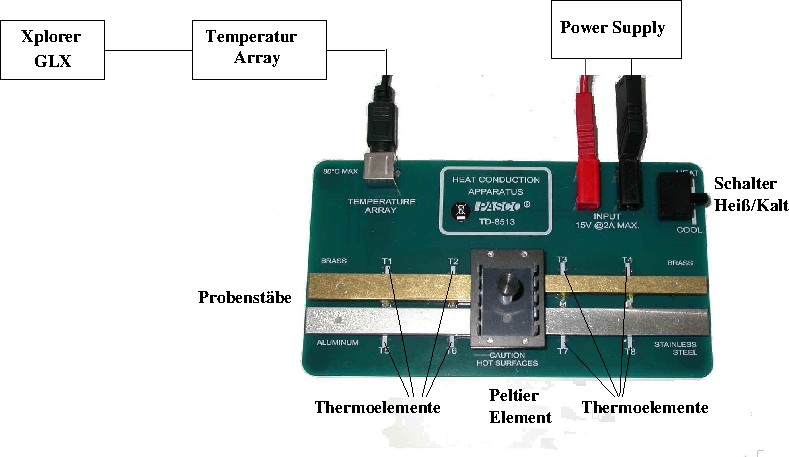
\includegraphics[width=0.5\textwidth]{build/Abb_1.pdf}
    \caption {Schematische Darstellung eines Lock-In-Verstärkers\cite[1]{V303}.}
    \label{fig:Abb_1}
\end{figure}
Im Folgenden wird der Lock-In-Verstärker schematisch mit \autoref{fig:Abb_1} erklärt.
Das Nutzsignal $U_{sig}$, was moduliert und verrauscht ist, wird durch einen Bandpassfilter zu einem Mischer geleitet.
Der Bandpassfilter befreit das Signal von Frequenzen, die viel größer sind als die Referenzfrequenz $(\omega >> \omega_0)$ und die viel kleiner $(\omega << \omega_0)$ sind.
Außerdem wird ein Referenzsignal $U_{ref}$ durch einen Phasenschieber zum Mischer geleitet.
Mit dem Phasenschieber kann die Phase des Referenzsignals variiert werden und mit dem Nutzsignal synchronisiert werden.
Die beiden Spannungen werden im Mischer mit der Frequenz $\omega_0$ multipliziert und es entsteht ein Mischsignal $U_{sig} \texttimes U_{ref}$.
Dieses wird im nachgeschalteten Tiefpassfilter über mehrere Perioden der Modulationsfrequenz integriert, sodass Rauschbeiträge herausgemittelt werden, die nicht zur Modulationsfrequenz synchronisiert sind.
Durch diesen Aufbau kann eine Güte von $Q = 10^6$ erreicht werden, wobei ein normaler Bandpass im Vergleich eine Güte von $Q=10^3$ erreicht.\\
Im Allgemeinen wird das Referenzsignal $U_{ref}$ als Rechteckspannung realisiert, was durch eine Fourier-Reihe angenähert werden kann zu
\begin{equation}
    U_{ref} =\frac{4}{\pi}\Bigl( \text{sin}(\omega t) + \frac{1}{3}\text{sin}(3\omega t) + \frac{1}{5}\text{sin}(5\omega t) + ... \Bigr).
    \label{eqn:Referenzsignal}
\end{equation}
Zusammen mit dem sinusförmigen Nutzsignal
\begin{equation}
    U_{sig} = U_0 \text{sin}(\omega t)
    \label{eqn:Nutzsignal}
\end{equation}
ergibt sich das Produkt
\begin{equation}
    U_{sig} \texttimes U_{ref} = \frac{2}{\pi} U_0 \Bigl(1-\frac{2}{3}\text{cos}(2\omega t)-\frac{2}{15}\text{cos}(4\omega t)-\frac{2}{35}\text{cos}(6\omega t)+...\Bigr).
\end{equation}
Dies enthält die geraden Oberwellen der Grundfrequenz $\omega$.
Die Ausgangspannung 
\begin{equation}
    U_{out} = \frac{2}{\pi} U_0
\end{equation}
wird durch den Tiefpassfilter so angeglichen, dass sie proportional zur Signalspannung ist.
Bei einer festen Phasendifferenz ergibt sich die Ausgangspannung
\begin{equation}
    U_{out} = \frac{2}{\pi}U_0 \text{cos}(\phi),
\end{equation}
welche auch maximal bei $\phi = 0$ ist.
